\documentclass[aspectratio=169,10pt]{beamer}
\usetheme{Boadilla}
\usepackage{graphicx,booktabs}
\title{Which backgrounds should train the next BDT?}
\subtitle{v3 signal and full Zbb/Zcc/Zss feature comparison; fixed 1,091-chunk model}
\author{FCC-ee $\Lambda_b\to\Lambda\gamma$ analysis}
\date{4 October 2026}
\begin{document}
\frame{\titlepage}

\begin{frame}{Question and denominators}
\begin{itemize}
\item Compare v3 offline-selected direct signal to nonmatched Zbb, Zcc and Zss before a mixed-background BDT is trained.
\item Zbb: 1,091 chunks and 395,623,929 input events; Zcc: 1,200 and 499,786,495; Zss: 1,200 and 499,842,440.
\item Signal: 100,002 generated direct decays in 100,000 events. Both charge conjugates included.
\item Offline selection: $\Lambda$ mass $\pm12.5$ MeV, $\Lambda_b$ energy $\geq10.5$ GeV, same hemisphere. Peak: reconstructed 5.4--5.9 GeV.
\item Feature figures normalize each candidate class separately. Yield figures use $6\times10^{12}$ Z and separate processed-event denominators.
\end{itemize}
\end{frame}

\begin{frame}{Observed candidate rows and projected peak}
\small
\begin{tabular}{lrrrr}
\toprule
Class & Offline rows & BDT rows & Final peak rows & Expected final peak\\
\midrule
Direct $\Lambda_b\to\Lambda\gamma$ & 54,872 & 37,802 & 23,849 & 194,757\\
Nonmatched Zbb & 1,113,719 & 528 & 27 & 61,422\\
Nonmatched Zcc & 1,834,608 & 1,720 & 252 & 363,943\\
Nonmatched Zss & 2,161,759 & 4,577 & 514 & 962,511\\
\bottomrule
\end{tabular}
\vspace{1em}

\small Final means fixed score $\geq0.9538269639$ plus the proposed Armenteros, $\pi^0$ and $\eta$ vetoes. The final projected inclusive peak background is 4.4\% Zbb, 26.2\% Zcc, 69.4\% Zss under the stated Z branching scenario. These are candidate rows, not collision counts.
\end{frame}

\begin{frame}{Existing Zbb-trained score tail}
\centering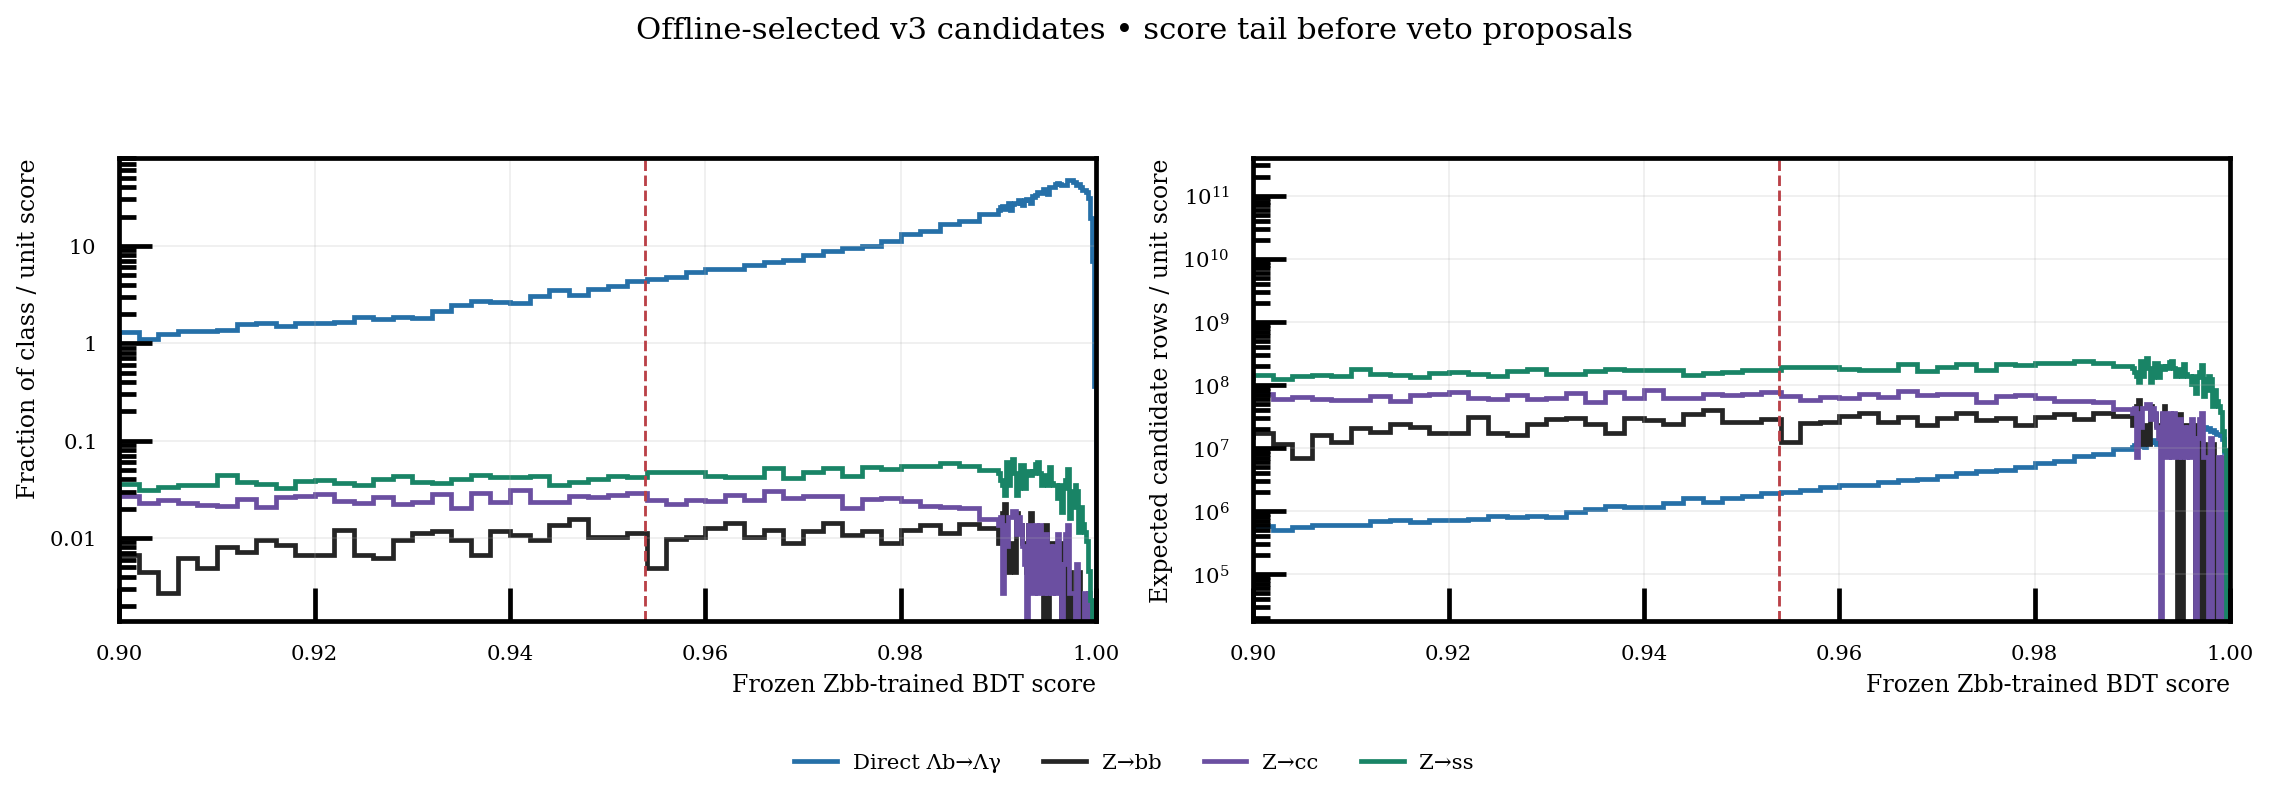
\includegraphics[width=.96\textwidth,height=.79\textheight,keepaspectratio]{figures/pre_bdt_score_tail.png}
\end{frame}

\begin{frame}{Peak-window kinematics before BDT}
\centering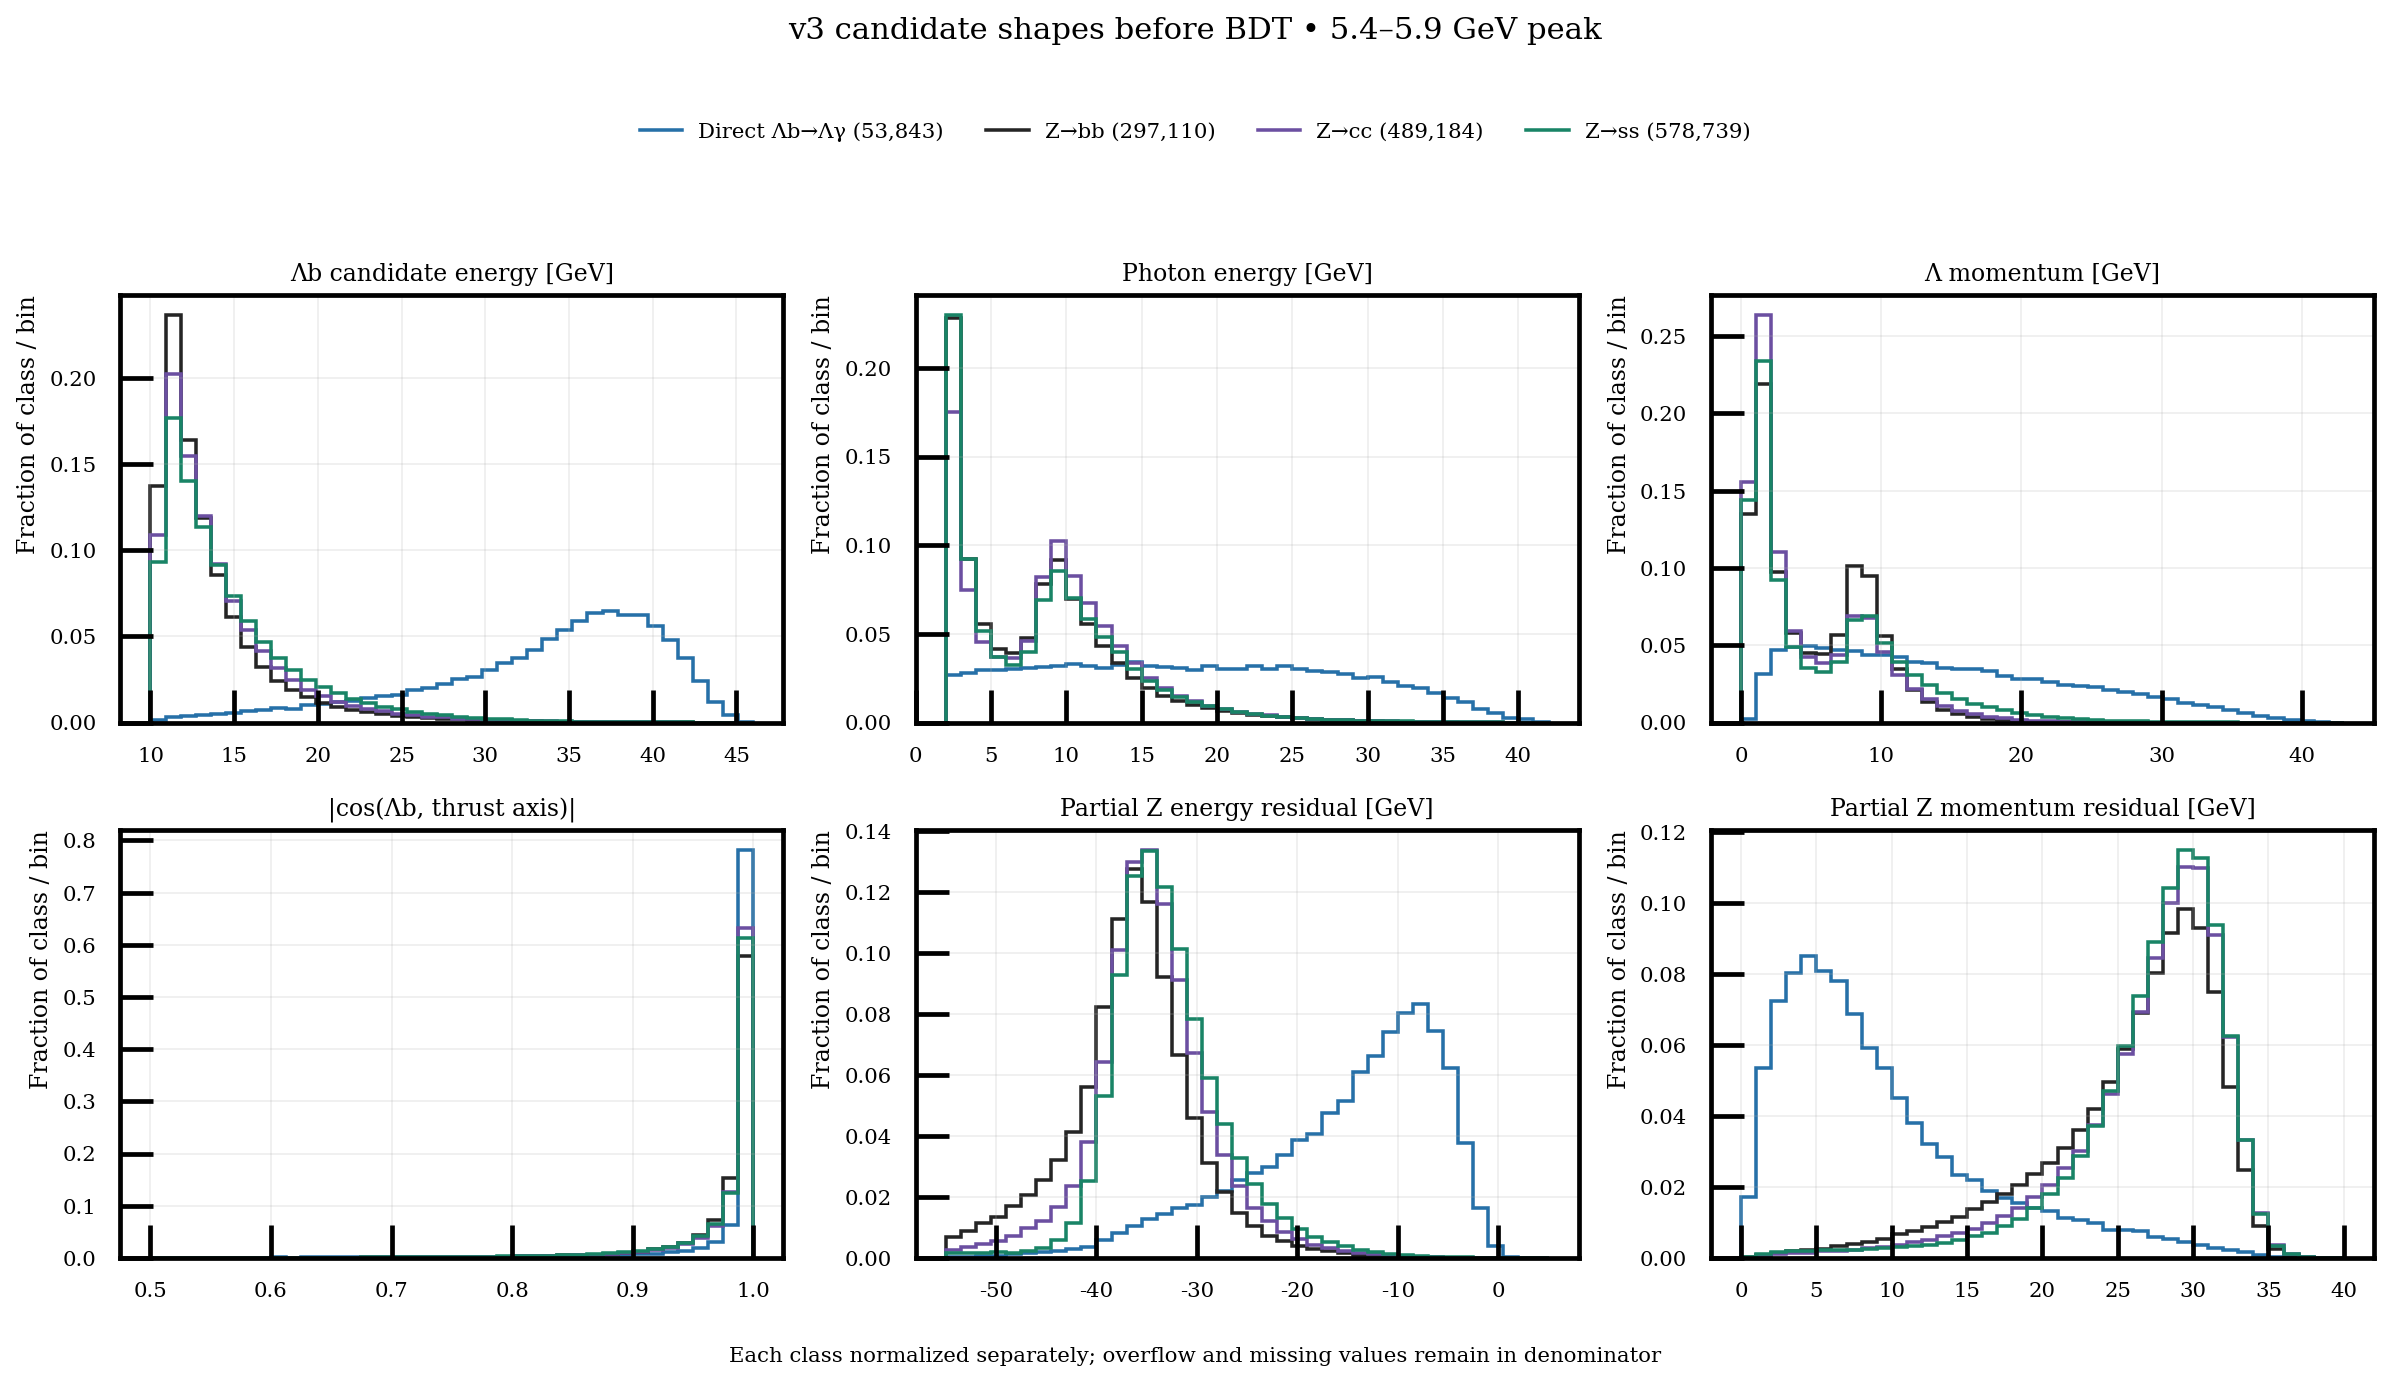
\includegraphics[width=.96\textwidth,height=.81\textheight,keepaspectratio]{figures/pre_bdt_peak_kinematics.png}
\end{frame}

\begin{frame}{Peak-window topology before BDT}
\centering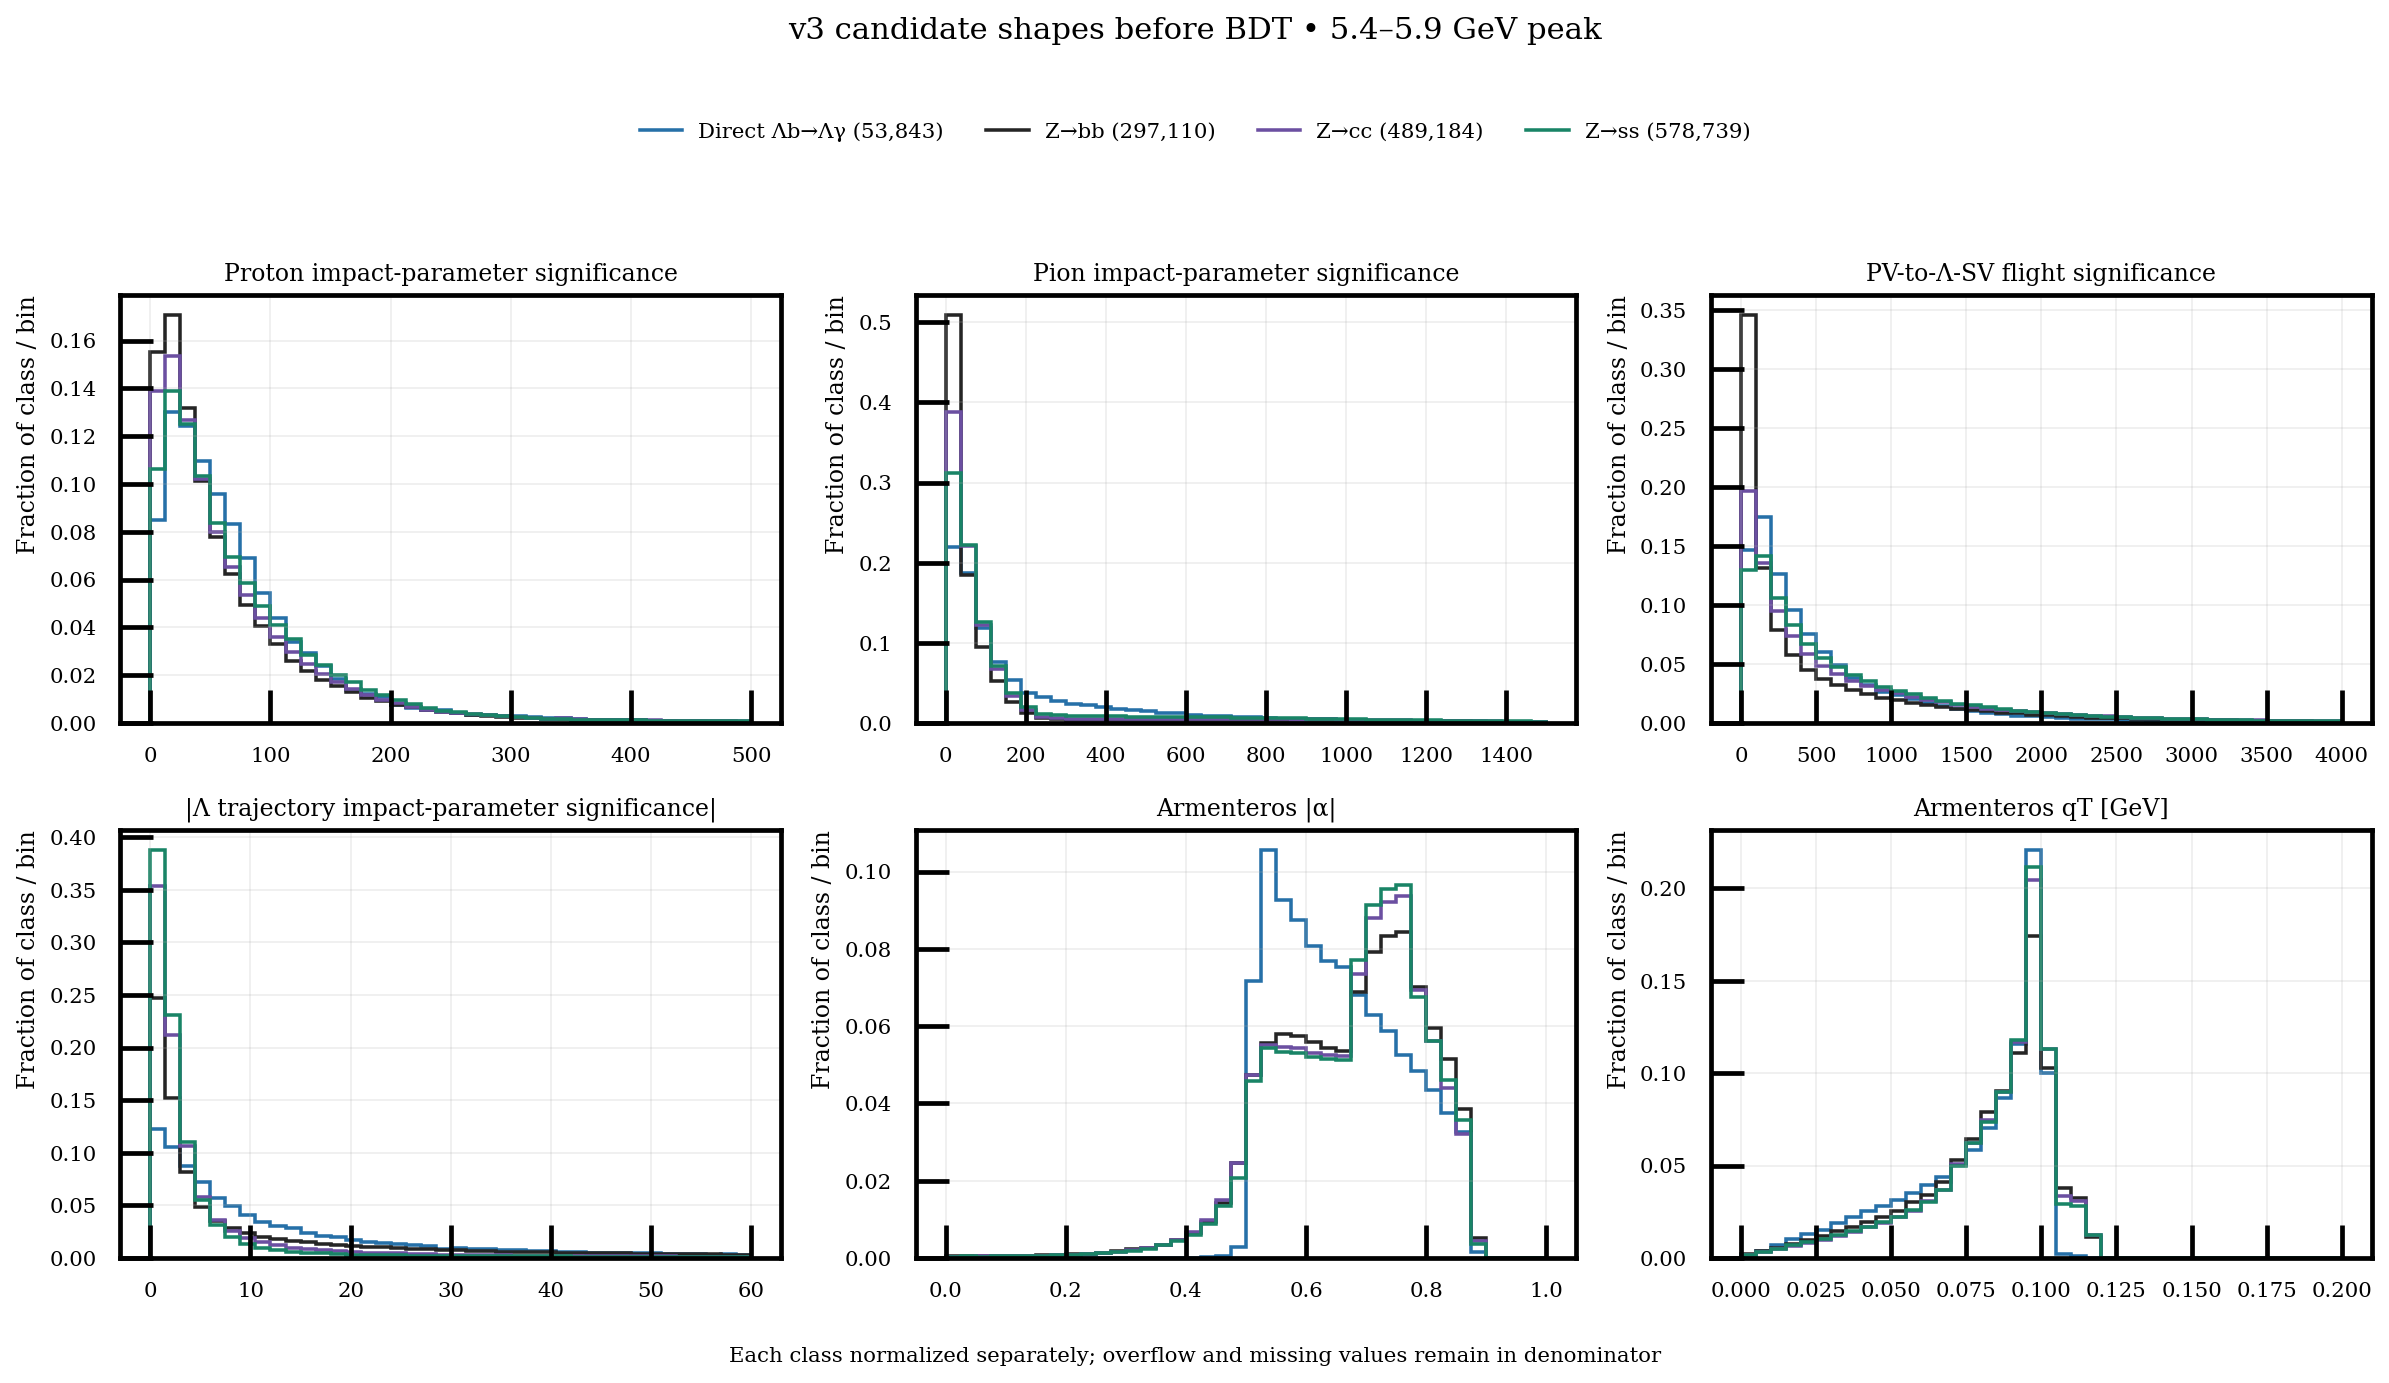
\includegraphics[width=.96\textwidth,height=.81\textheight,keepaspectratio]{figures/pre_bdt_peak_topology.png}
\end{frame}

\begin{frame}{Peak-window isolation and photon pairing}
\centering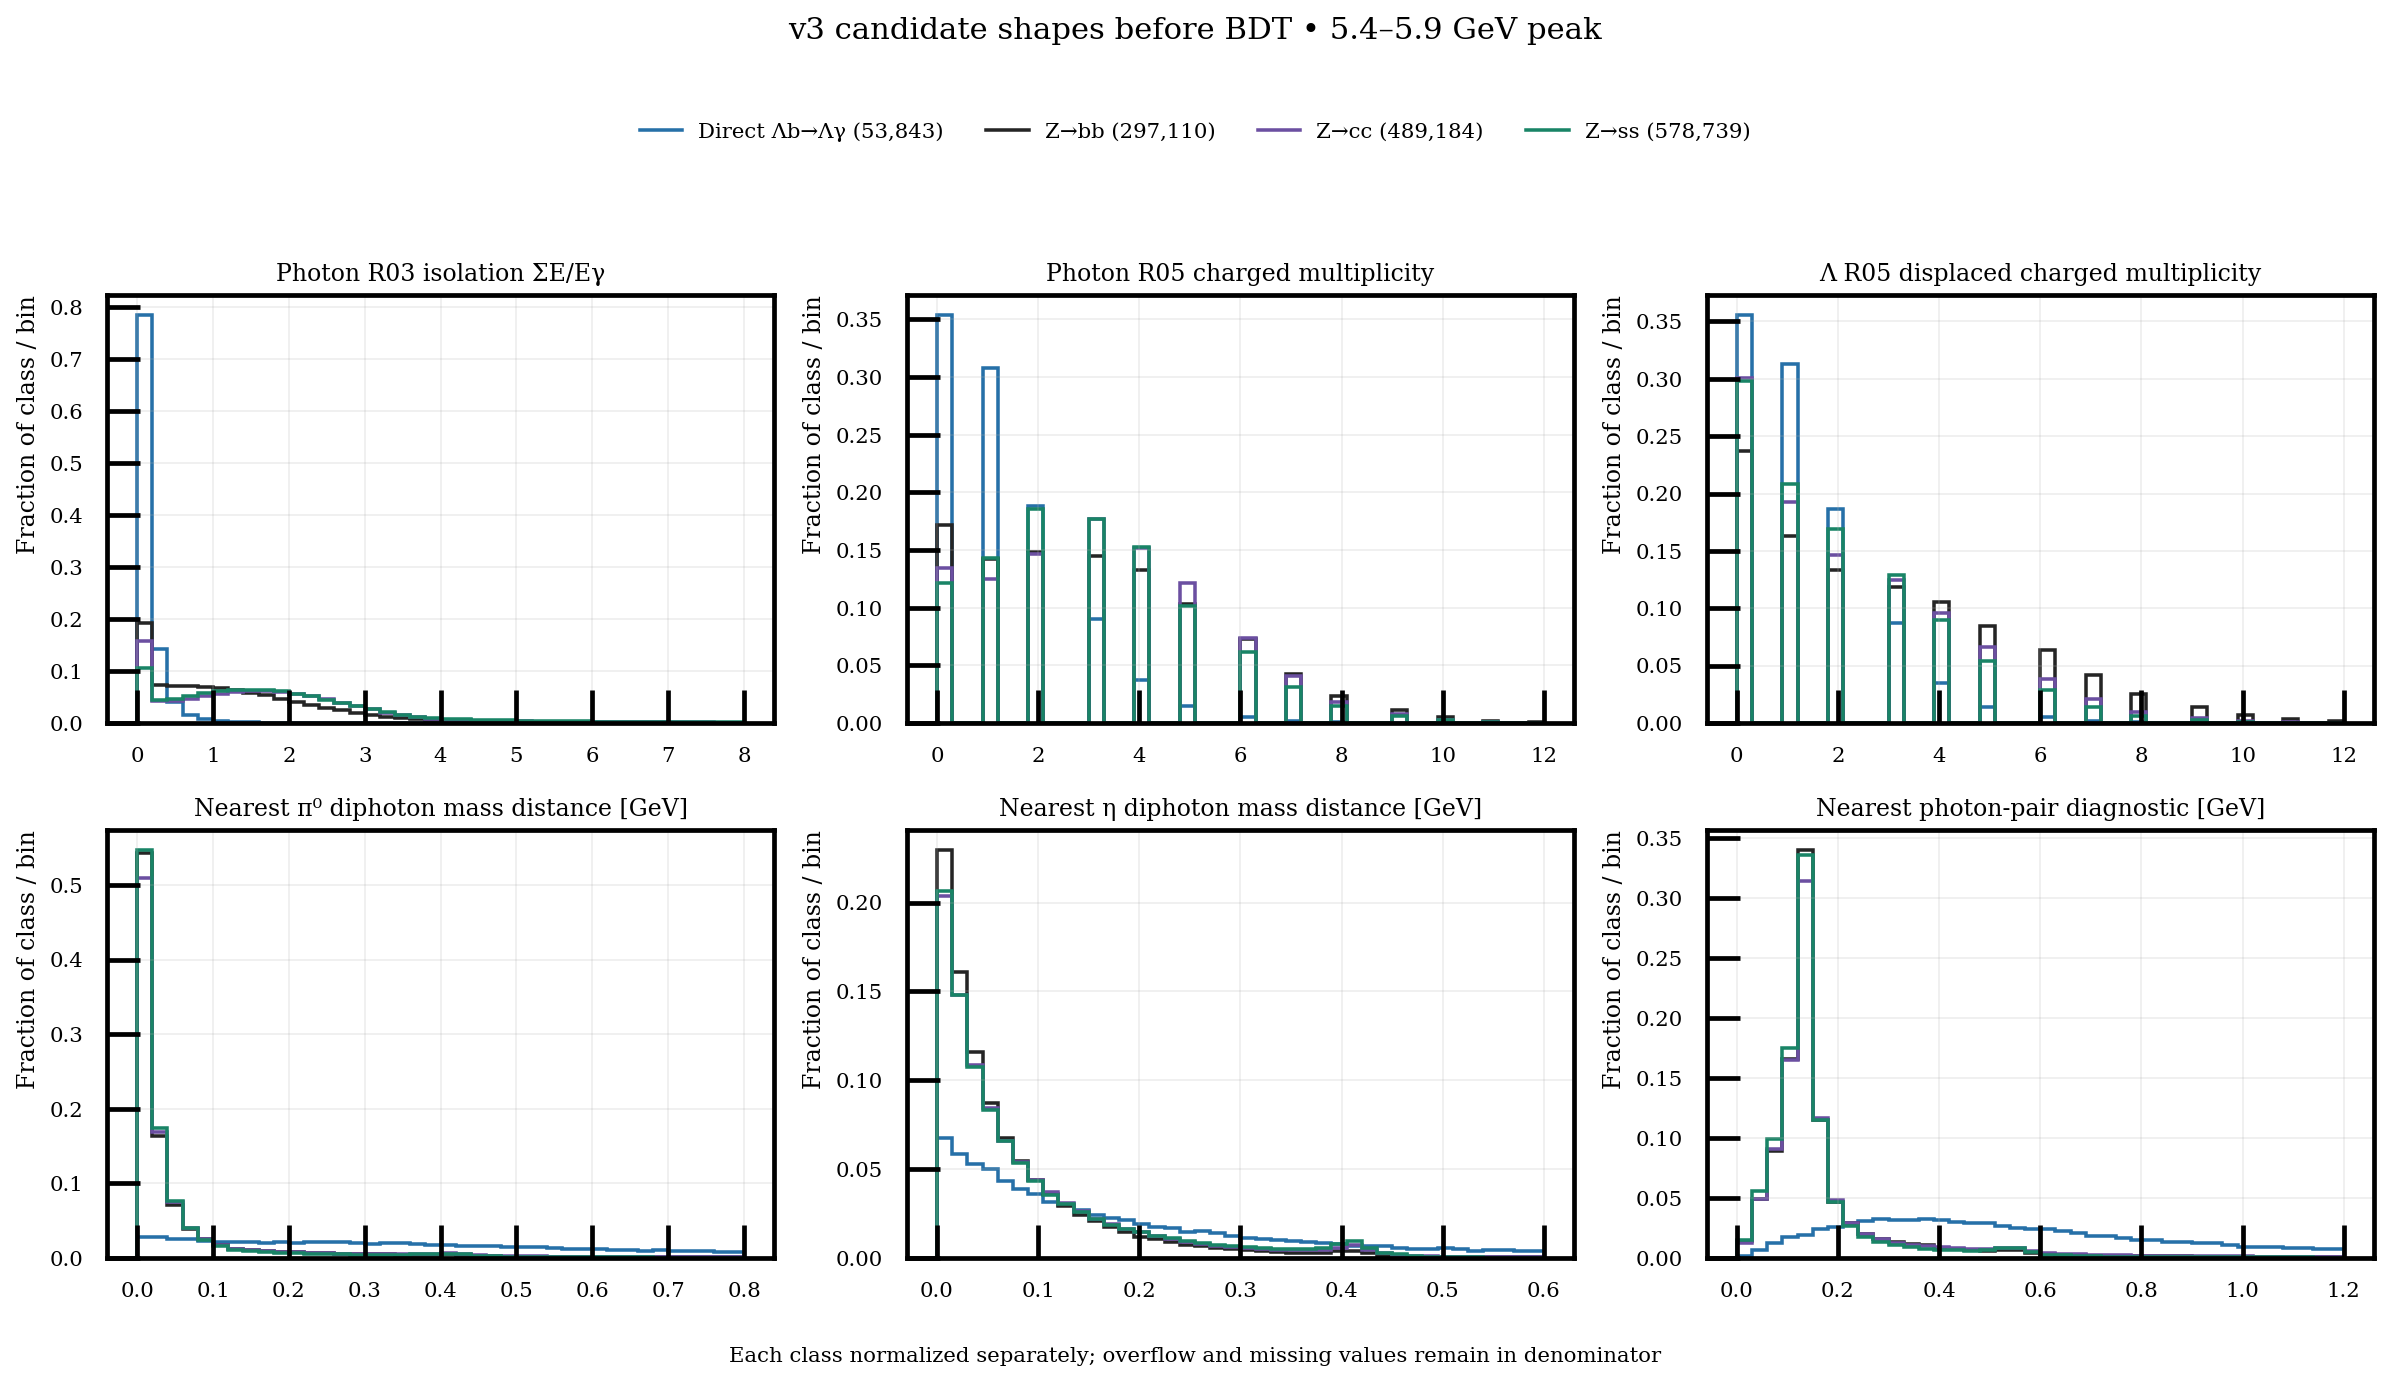
\includegraphics[width=.96\textwidth,height=.81\textheight,keepaspectratio]{figures/pre_bdt_peak_activity.png}
\end{frame}

\begin{frame}{Topology in the current surviving tail}
\centering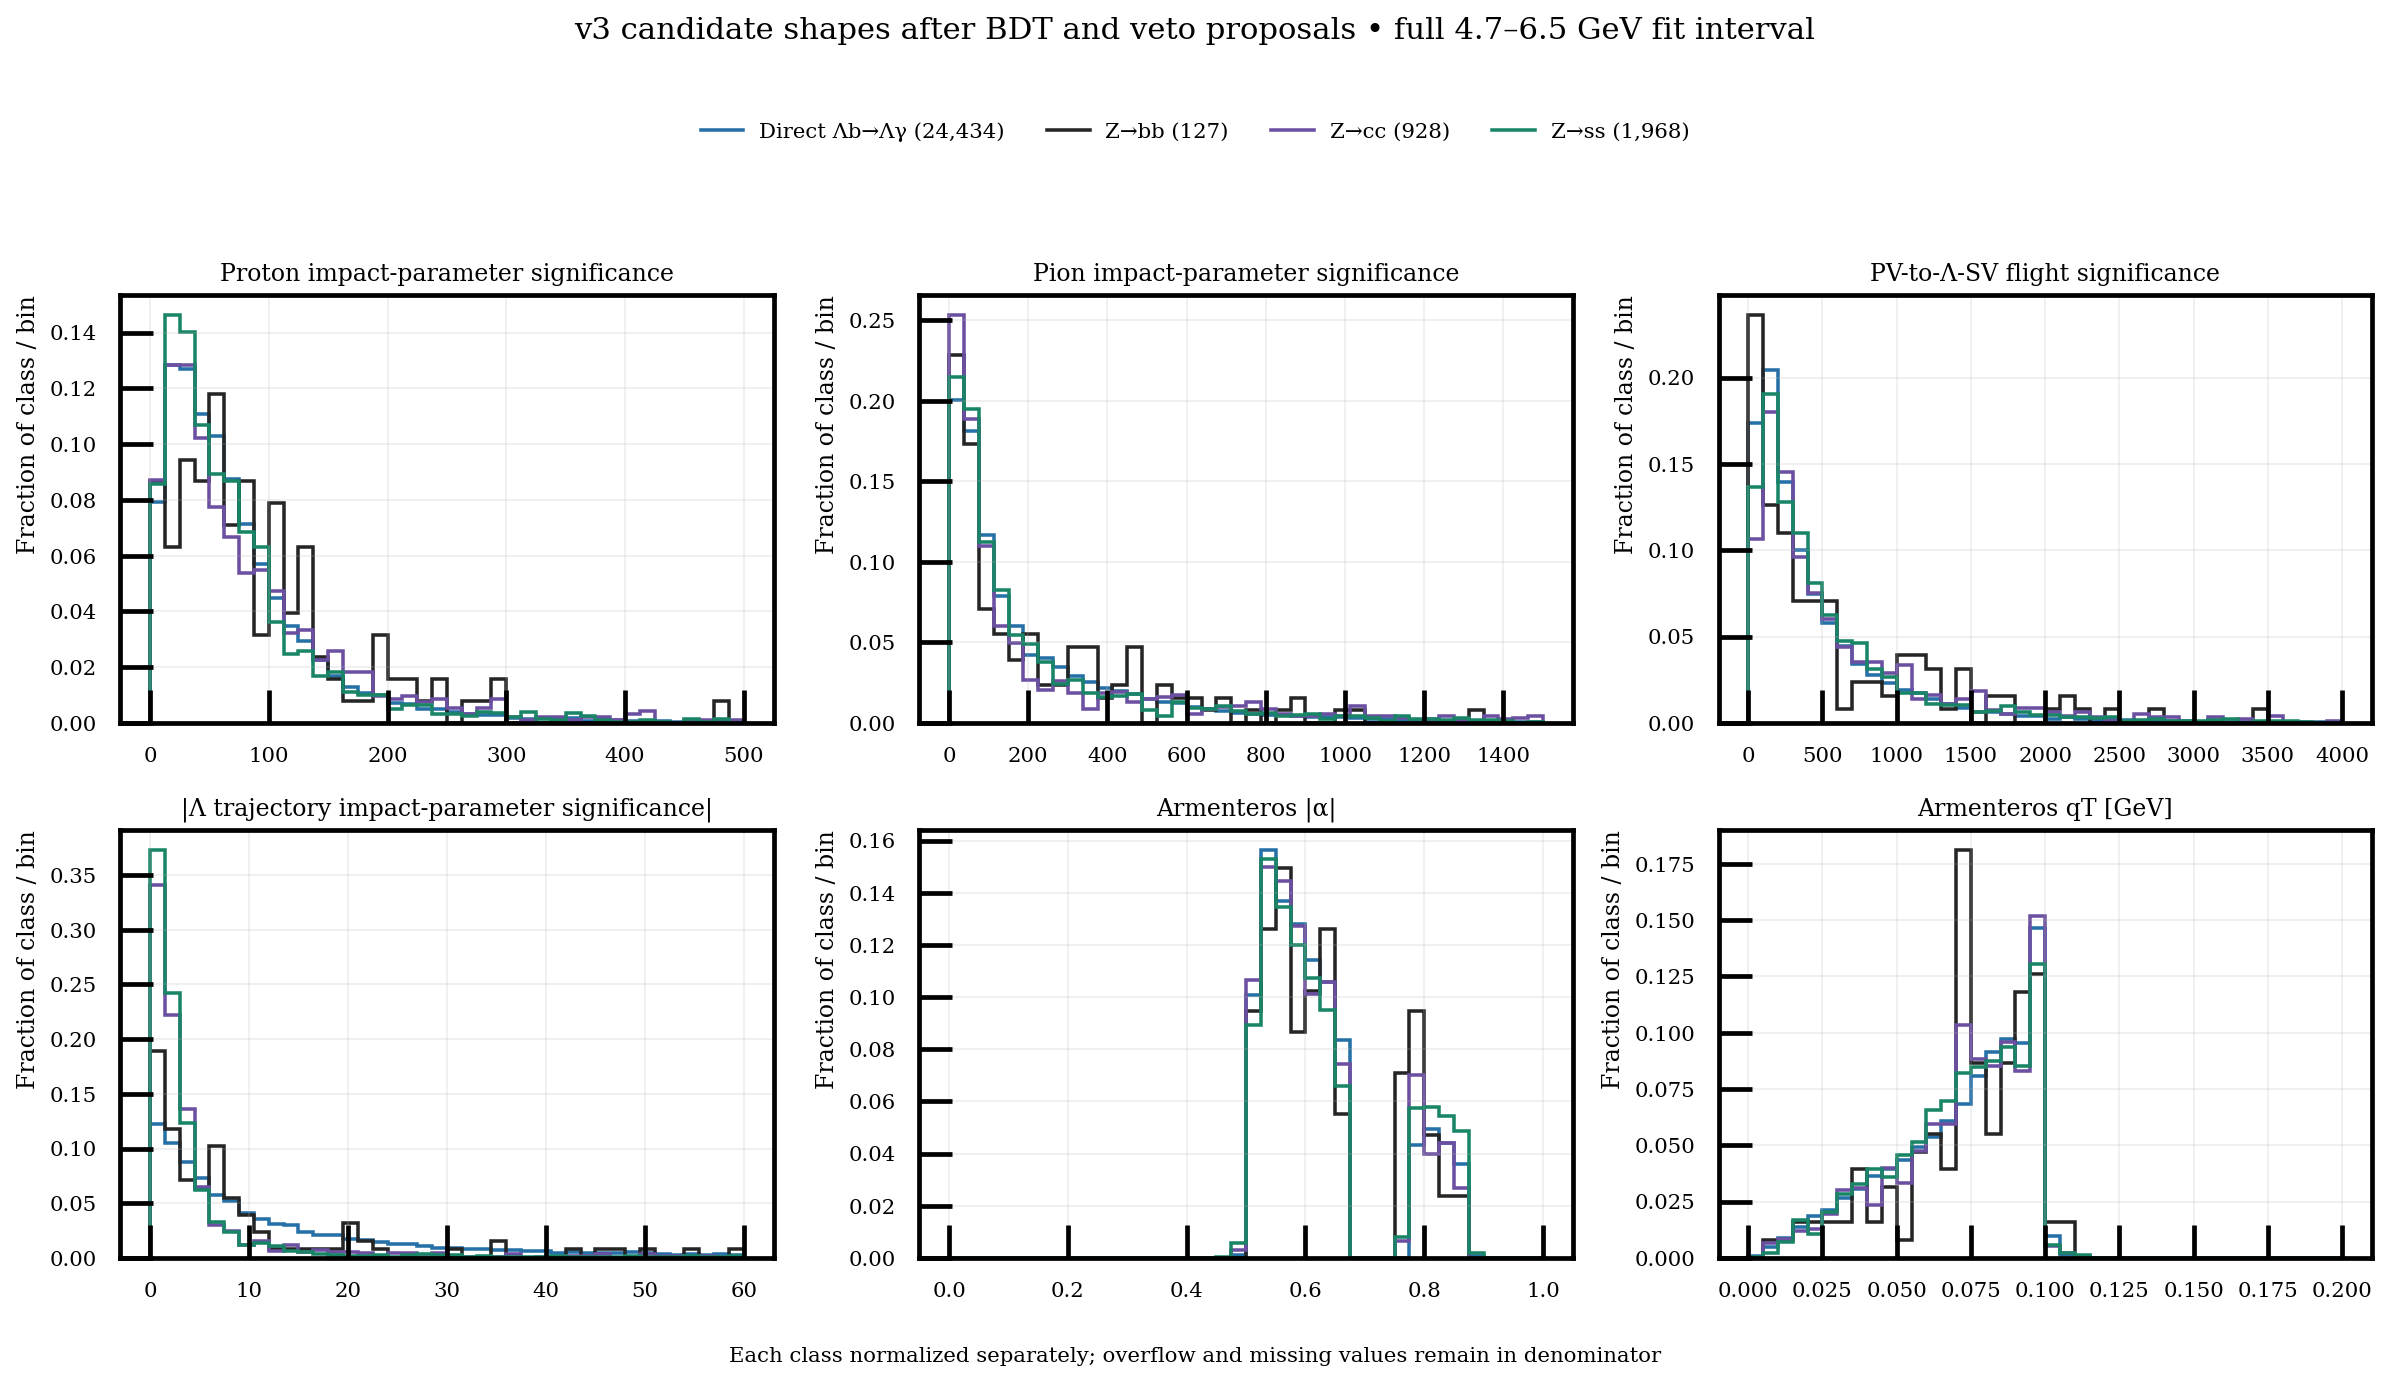
\includegraphics[width=.96\textwidth,height=.81\textheight,keepaspectratio]{figures/post_bdt_vetoes_topology.png}
\end{frame}

\begin{frame}{Final expected mass and angle on a linear scale}
\centering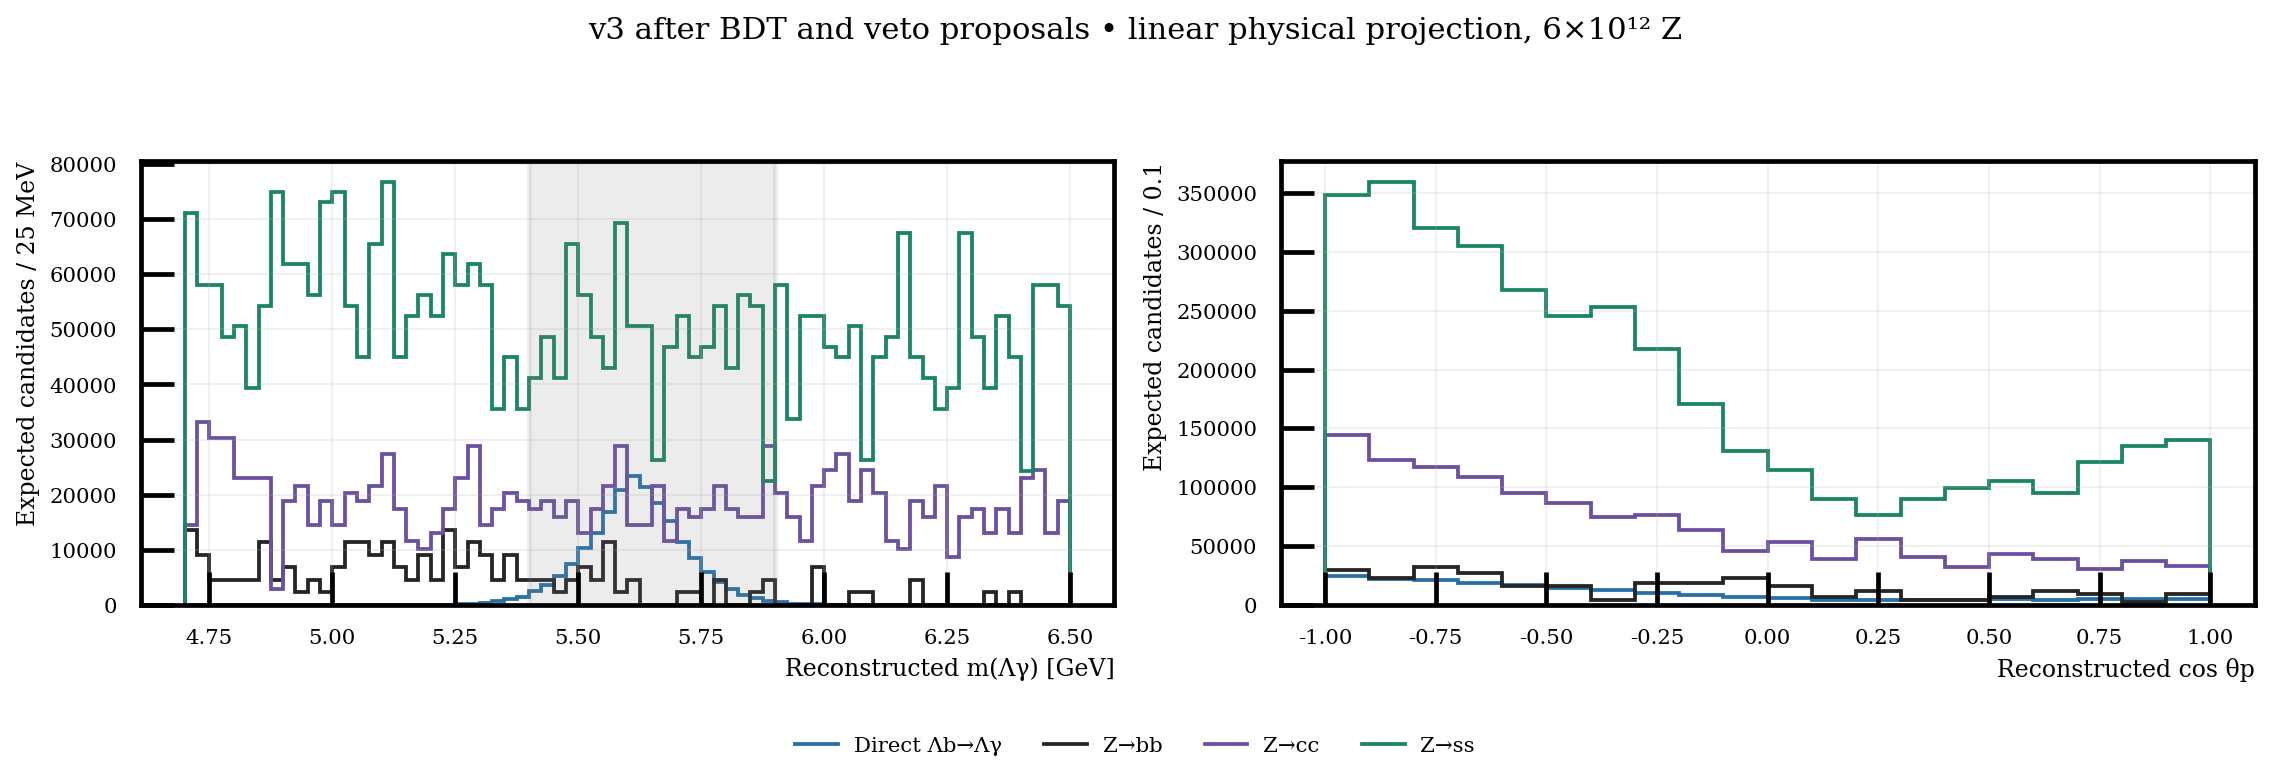
\includegraphics[width=.96\textwidth,height=.79\textheight,keepaspectratio]{figures/post_bdt_vetoes_mass_angle_linear.png}
\end{frame}

\begin{frame}{Proposed controlled model comparison}
\begin{itemize}
\item Compare the same 20 features with Zbb-only training and with a physically motivated Zbb/Zcc/Zss background mixture.
\item Add reconstructed $|d_0(\Lambda)/\sigma|$ as a separate mixture-model ablation. It is absent from the current 20 features; its peak marginal TV from signal is 0.415 for Zss versus 0.189 for Zbb.
\item Keep Armenteros $\alpha,q_T$ as a separate test. Existing energy, recoil and isolation features already carry strong signal/background separation.
\item Freeze train/validation/test by event and production chunk. Optimize $S/\sqrt{S+B}$ in the peak on validation, then check per-flavour tails, mass/angle and PHSP acceptance on held-out data.
\item These plots are descriptive and include existing Zbb training chunks. No mixed model or new feature is adopted here.
\end{itemize}
\end{frame}
\end{document}
